\subsection{Receiver Pointing}
For the pointing of the receiver instrument three options are considered. The first concept is pointing the entire satellite towards the Earth using an active \ac{ACS}. Using this system will also influence the behaviour of the solar cells, since the solar cells will move as well along with the satellite. The second concept is using two stepper motors for moving the instrument only. This concept will allow the instrument to move independently from the satellite, but will add more mass and moving parts to the satellite. Concept number three is a hybrid system. The rotation along the yaw-axis of the satellite is done by rotation the satellite, while the rotation along the other two axis is done using a single stepper motor. This way the satellite and the instrument can move semi-independent from each other and look at both the ground target and the Sun. Schematics of the different options are shown in figure \ref{fig:pointeroptions} on page \pageref{fig:pointeroptions}.

\begin{figure}[h]
\centering
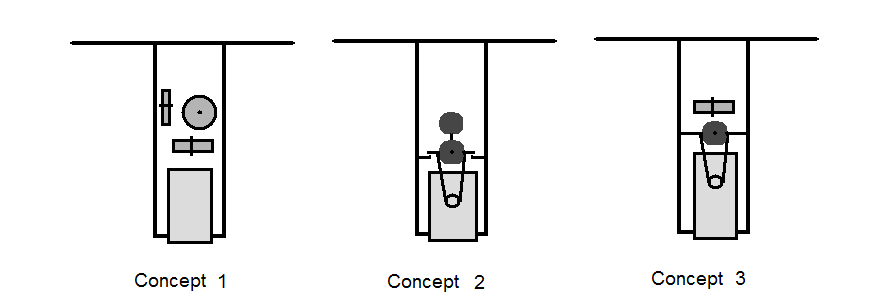
\includegraphics[width=0.8\textwidth, bb=0 0 895px 298px]{img/pointingsystemoptions.png} 
\label{fig:pointeroptions}
\caption[Design options for the pointing mechanism]{Design options for the pointing mechanism. The first option uses only the \ac{ACS}, the second option only mechanical actuators, the third option is a combination of both using the \ac{ACS} for the yaw-axis and a mechanical actuator for the other axis. The light grey box represents the instrument, one shade darker are reaction wheels and the dark boxes are actuators.}
\end{figure}

The trade-off criteria used are pointing accuracy, pointing rate, added weight, reliability, power, influence on other subsystems and the system complexity. Because the instrument can not work if the satellite is not pointed towards the ground target the pointing accuracy and pointing rate are given a weight factor of 5. The complexity, reliability and influence on other subsystems are less important comparably since the swarm is used for redundancy in making measurements and other subsystems can be adapted to meet their requirements, a weight factor of 3 is given. The weight and power use of the system is given a factor of 2, because it is important for the satellite as a whole, but not the main driver for the mission.

\begin{table} [h]
\centering
\begin{tabular}{p{3cm} | c | c c c}
\textbf{Criteria} & \textbf{Weight Factor} & \textbf{Concept 1} & \textbf{Concept 2} & \textbf{Concept 3} \\ \hline \hline
Pointing accuracy & 10 & 2 & 8 & 6 \\
Pointing rate     & 10 & 2 & 8 & 6 \\
Added weight      & 4  & 8 & 2 & 5 \\
Reliability       & 6  & 8 & 3 & 7 \\
Power             & 4  & 7 & 2 & 4 \\
Influence         & 6  & 2 & 5 & 7\\
Complexity        & 6  & 8 & 2 & 5 \\ \hline
Weighted total    &    & 208 & 233 & 222
\end{tabular} 
\caption[Trade-off pointing mechanism]{Trade-off graph for the pointing mechanism. The weight factor signifies the importance of the criterion. Grades are given on a scale of 1 to 10, 1 being the worst, 10 the best}
\label{tab:pointingtradeoff}
\end{table}

Table \ref{tab:pointingtradeoff} on page \pageref{tab:pointingtradeoff} shows the numerical values assigned to the different criteria. 
Pointing with only stepper motors can be done the most precise, the combination with a reaction wheel for the yaw-axis the precision around that axis will be lower, using only the \ac{ACS} the accuracy will be the lowest. 
Stepper motors are able to respond really quickly, the reaction wheel option takes a lot longer to respond, since it has to move the entire satellite, not just a part. The pointing speed for the hybrid system will be somewhere in between, but will be better than average given the change in ground elevation will be larger than the change in relative position of the emitter.
When the entire satellite is turned almost almost no extra mass need to be added, since attitude control is needed in the satellite anyway. With two actuators the two extra masses are added to the structure. In the hybrid concept only one additional actuator has to be taken.
Since no additional parts are added to the system at concept one, the reliability of the concept will be just as high as the entire \ac{ADCS}. Using only actuators adds two moving parts to the satellite and moving parts always add risk to spacecraft. Although the hybrid system only adds one moving part, it is still less reliable than none.
Although concept one uses the existing \ac{ACS} still a little more power is needed to make the manoeuvres for pointing towards the ground target. Stepper motors use power and two use more than one.
Turning the entire satellite will mostly effect the other subsystems, e.g. the solar panels need to be pointed towards the Sun and the atmospheric drag will change throughout the orbit putting an extra load on the \ac{AOCS}. The second concept will add much mass to the satellite, not only for the motors, but also for the support structure. This will lead to more launch mass and more fuel needed to keep the satellite in orbit. The third concept will also add mass, but less the second concept. In the latter two cases the solar panels still can be pointed towards the Sun, if required.
The \ac{ACS} will need to be made more precise for the concept to work, also the control algorithms will need to be very advanced. A lot more structure has to be added to the satellite in option two to make the satellite move in both directions. For concept three also some extra structure need to be added, but far less than with concept two. Also extra communication with the \ac{ADCS} is required.

Concept number one is the clear loser in this trade-off. Concepts two and three are much closer together. Concept two scores high at the pointing accuracy and rate, but rather low scores for the rest, while concept three scores average overall. 
Concept number three is chosen, because of its slightly better overall score.